\documentclass[]{article}
\usepackage{url}
\usepackage{cite}
\usepackage{listings}
\usepackage{xcolor} % for setting colors
\usepackage{lmodern}
\usepackage{graphicx}
\usepackage{textcomp}
\usepackage{hyperref}
\usepackage{enumerate}
\usepackage[numbers]{natbib}	

% set the default code style
\lstset{
	frame=tb, % draw a frame at the top and bottom of the code block
	tabsize=4, % tab space width
	showstringspaces=false, % don't mark spaces in strings
	numbers=left, % display line numbers on the left
	commentstyle=\color{green}, % comment color
	keywordstyle=\color{blue}, % keyword color
	stringstyle=\color{red} % string color
}

%opening
\title{Volentix network v0.0.1}
\author{
		Sylvain Cormier\\
	\texttt{sylvain@volentixlabs.com}
}


\begin{document}

\maketitle

\begin{abstract}

The Volentix token, VTX was originally created on the main EOSIO chain.
The Volentix network is a network of voting nodes which run software to support the volentix ecosystem:
Staking, Proposals and Wrapping of VTX on EOS/Ethereum. 

\end{abstract}

\section{Introduction }

	The Volentix network is a docker network using a .yml file for configuration.

\section{System}
\begin{enumerate}
	\item \textbf{Docker network } \\
	\begin{enumerate}
	\item An oracle script\
	constantly feeding an EOS contract with the ETH VTX balance, account name, timestamp, and block info* (disabled in this version ) 
	\item OpenEthereum
	\item Bitcoin
	\item EOS
	\item Volentixnode \
	\begin{enumerate}
		\item Voting
		\item Distribution
		\item Signing (Disabled in this version)
	\end{enumerate}
\end{enumerate}
		\item \textbf{Registration} \\
			User chooses jobs:
				\begin{enumerate}  
					\item Voting system(mandatory)
					\item Oracle
				\end{enumerate}
		\item \textbf{EOS contracts} \
		\begin{enumerate}  
			\item Staking
			\item Custodian
			\item Token
			\item Pool
			\item Gateway
		\end{enumerate}
		
\end{enumerate}
 
\begin{figure}
	centering
	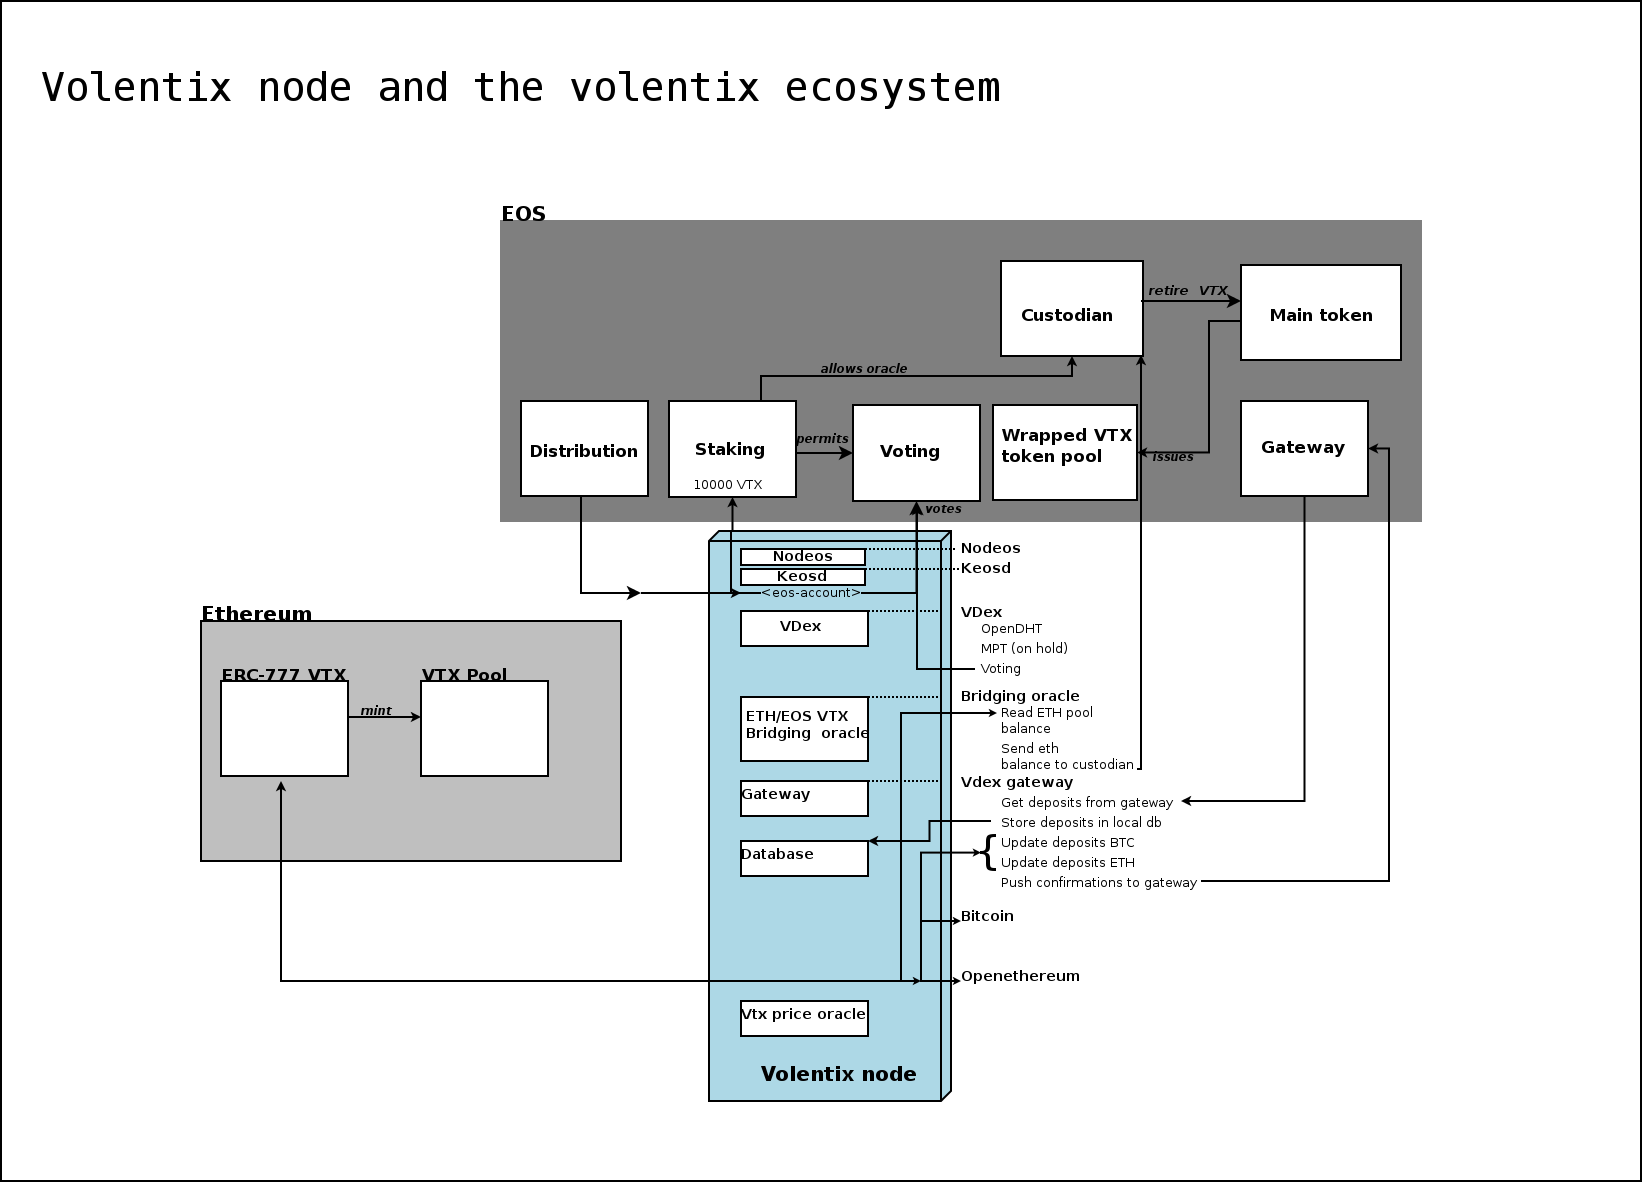
\includegraphics[scale=0.2]{vltxnode.png}
	\caption{}
	\label{fig:whitebackground-ecosystem02}
\end{figure}

\section{Conditions}
\begin{enumerate}
	\item EOS custodian must be  must be updated continuously by a minimum of 8 oracles.
	\item No oracle can submit its value twice. 
	\item Sources must register to the Volentix node network.
	\item Users must be able to pick the work/rewards they do.
	\item Volentix nodes should be extended with new functionality of being able to update  without having to null registrations.
	\item Nodes must have 10000 VTX staked. 	
\end{enumerate}
\end{document}
